% meta.concepts: 3D centroid
% meta.tags: centroid
% acknowledge: Engineering Statics: Open and Interactive
% source: Chapter 7 Example 7.5.3 of online edition (access: Feb. 13, 2023)

A composite solid consists of a rectangular block of lightweight concrete and a triangular wedge of steel with dimensions as shown. The rectangular block has a $2 ft$ radius circular hole, centered and drilled through its full depth, perpendicular to the front and back faces.

Assume:
\begin{itemize}
  \item $\gamma_C = 125 lb/ft^3$
  \item $\gamma_S = 493 lb/ft^3$
\end{itemize}

Find the center of mass of this composite solid.

\begin{figure}[ht!]
  \centering
  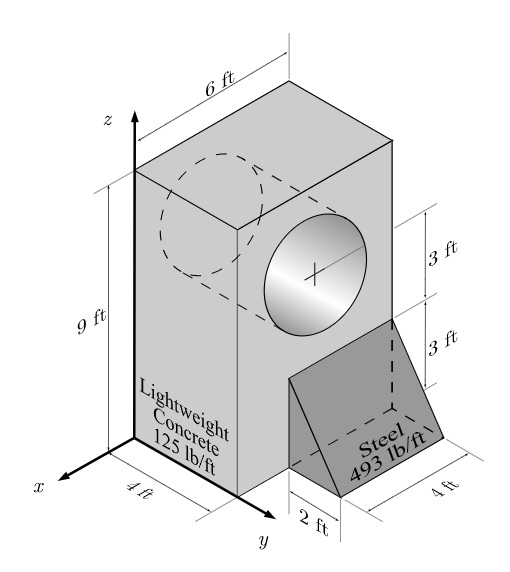
\includegraphics[width=0.4\textwidth,height=0.3\textheight,keepaspectratio]{fig.png}
\end{figure}

\iftoggle{flagSoln}{%
\vspace{.5cm}
\rule{\textwidth}{.4pt}
\vspace{.5cm}
\textbf{Solution:}
\begin{figure}[ht!]
  \centering
  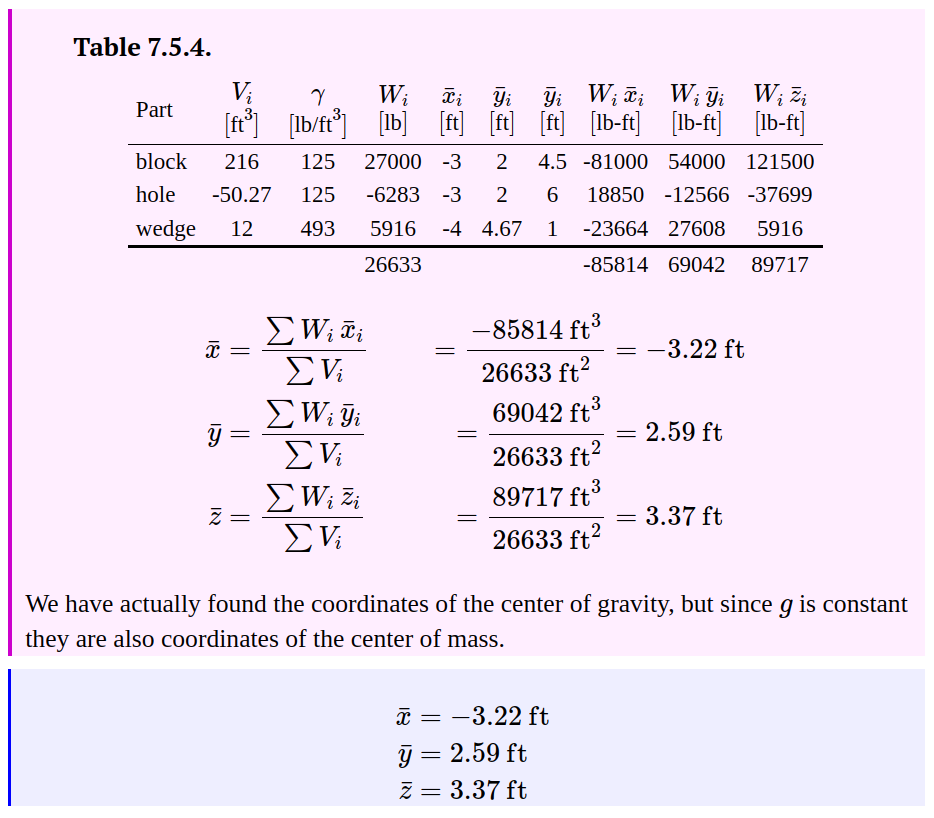
\includegraphics[width=0.9\textwidth,
	           height=0.4\textheight,
		   keepaspectratio]{soln.png}
\end{figure}
}{%
}%
